\documentclass[../main/main.tex]{subfiles}
\usetikzlibrary{trees}

%_______________________________________________________________________________________________________________________
\begin{document}
	
	
	
	
\section{Estrutura de dados da HiGtree}



%-------Slide 1-------	
%----------------------------------------------------------------------------------------------------------------------	
\setLayout{mainpoint}
\begin{frame}
	\frametitle{Estrutura de dados da HiGtree}
\end{frame}
%----------------------------------------------------------------------------------------------------------------------	




%-------Slide 2-------	
%----------------------------------------------------------------------------------------------------------------------	
\setLayout{vertical}
\begin{frame}
	\begin{block}{}
		A HiG-Tree (\textit{Hierarchical Grid Tree}) é uma estrutura de dados em árvore usada em malhas adaptativas, que permite refinamento, dividindo o espaço recursivamente, economizando memória e tempo de processamento.
	\end{block}
	
	\begin{block}{}
		Nos casos 2D e 3D, chamamos de \textit{quadtree} e \textit{octree}, respectivamente.
	\end{block}
\end{frame}
%----------------------------------------------------------------------------------------------------------------------	



%-------Slide 2-------	
%----------------------------------------------------------------------------------------------------------------------	
\setLayout{vertical}
\begin{frame}{\smaller \smaller Exemplo de HiG-Tree}
	\vspace{-1cm}
	\begin{center}
		\resizebox{0.3\textwidth}{!}{
			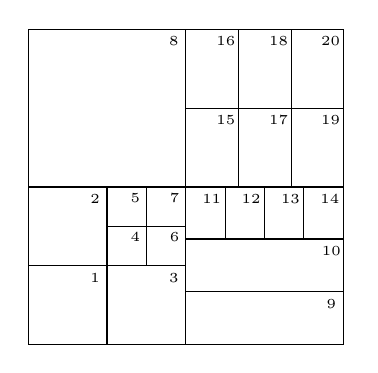
\begin{tikzpicture}[scale=1]
				
				\draw (0,0) rectangle (4,4);
				\draw (2,2) rectangle (4,4);
				\draw (0,0) rectangle (2,2);
				
				\draw (0,0) rectangle (1,1);
				\draw (0,1) rectangle (1,2);
				\draw (1,0) rectangle (2,1);
				\draw (1,1) rectangle (1.5,1.5);
				\draw (1.5,1.5) rectangle (2,2);
				
				\draw (2,2) rectangle (2.67,3);
				\draw (2.67,2) rectangle (3.34,3);
				\draw (3.34,2) rectangle (4,3);
				
				\draw (2,3) rectangle (2.67,4);
				\draw (2.67,3) rectangle (3.34,4);
				\draw (3.34,3) rectangle (4,4);
				
				\draw (2,0) rectangle (4,0.67);
				\draw (2,0.67) rectangle (4,1.34);
				\draw (2,1.34) rectangle (2.5,2);
				\draw (2.5,1.34) rectangle (3,2);
				\draw (3,1.34) rectangle (3.5,2);
				
				% Numerando os retângulos
				\node at (0.85,0.85) {\tiny 1};
				\node at (0.85,1.85) {\tiny 2};
				\node at (1.85,0.85) {\tiny 3};
				\node at (1.36,1.36) {\tiny 4};
				\node at (1.36,1.86) {\tiny 5};
				\node at (1.86,1.36) {\tiny 6};
				\node at (1.86,1.86) {\tiny 7};
				\node at (1.85,3.85) {\tiny 8};
				\node at (3.85,0.52) {\tiny 9};
				\node at (3.85,1.19) {\tiny 10};
				\node at (2.33,1.85) {\tiny 11};
				\node at (2.83,1.85) {\tiny 12};
				\node at (3.33,1.85) {\tiny 13};
				\node at (3.83,1.85) {\tiny 14};
				\node at (2.51,2.85) {\tiny 15};
				\node at (2.51,3.85) {\tiny 16};
				\node at (3.18,2.85) {\tiny 17};
				\node at (3.18,3.85) {\tiny 18};
				\node at (3.84,2.85) {\tiny 19};
				\node at (3.84,3.85) {\tiny 20};
				
			\end{tikzpicture}
		}
		
		\vspace{0.2cm}
		
		\resizebox{0.8\textwidth}{!}{
			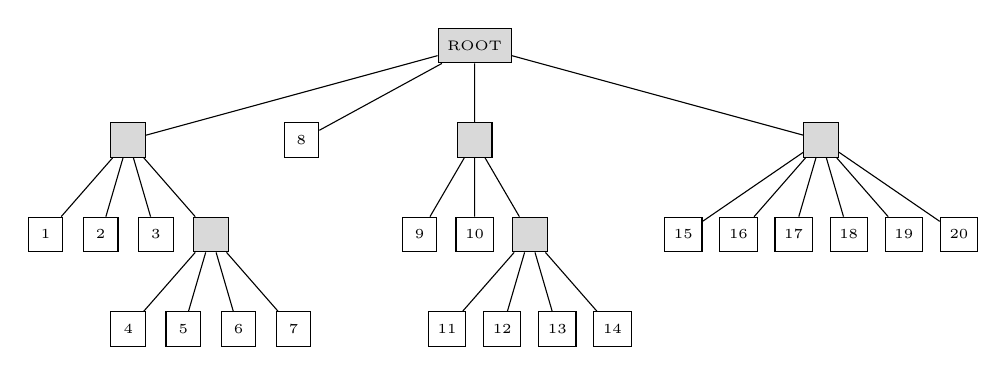
\begin{tikzpicture}[
				every node/.style={draw, rectangle, minimum size=4.4mm, align=center, font=\tiny},
				edge from parent/.style={draw,-},
				level distance=1.2cm,
				sibling distance=1.1cm,
				scale=1
				]
				
				\node[fill=gray!30] {ROOT}
				child {
					node[fill=gray!30] {}
					[sibling distance=7mm]
					child { node {1} }
					child { node {2} }
					child { node {3} }
					child { node[fill=gray!30] {}
						child { node {4} }
						child { node {5} }
						child { node {6} }
						child { node {7} }
					}
				}
				child[missing] {}
				child { node {8} }
				child[missing] {}
				child {
					node[fill=gray!30] {}
					[sibling distance=7mm]
					child { node {9} }
					child { node {10} }
					child { node[fill=gray!30] {}
						child { node {11} }
						child { node {12} }
						child { node {13} }
						child { node {14} }
					}
				}
				child[missing] {}
				child[missing] {}
				child[missing] {}
				child {
					node[fill=gray!30] {}
					[sibling distance=7mm]
					child { node {15} }
					child { node {16} }
					child { node {17} }
					child { node {18} }
					child { node {19} }
					child { node {20} }
				};
				
			\end{tikzpicture}
		}
		\captionof{figure}{Exemplo de malha 2D e sua \textit{quadtree} associada.}
	\end{center}
\end{frame}
%----------------------------------------------------------------------------------------------------------------------	



%-------Slide 3-------	
%----------------------------------------------------------------------------------------------------------------------	
\setLayout{vertical}
\begin{frame}[fragile]{\smaller \smaller Células da HiG-Tree}
	\begin{minipage}{0.45\textwidth}
		\begin{verbatim}
			typedef struct hig_cell {
				Point lowpoint; ------------
				Point highpoint; -----------
				int numcells[DIM]; ---------
				struct hig_cell * parent; --
				int posinparent; -----------
				struct hig_cell **children;-
				uniqueid ids[NUMIDS]; ------
			} hig_cell;
		\end{verbatim}
	\end{minipage}
	\hfill
	\begin{minipage}{0.45\textwidth}
		\vspace{-.1cm}
		$({x_1}_{min},{x_2}_{min},\cdots,{x_m}_{min})$
		
		$({x_1}_{max},{x_2}_{max},\cdots,{x_m}_{max})$
		
		$(n_1, n_2, \cdots, n_m)$
		\vspace{-.3cm}
		\begin{verbatim}
			célula-pai
			posição em relação ao pai
			células-filho
			id de cada célula/faceta
		\end{verbatim}
		
	\end{minipage}
\end{frame}
%----------------------------------------------------------------------------------------------------------------------	



%-------Slide 4-------	
%----------------------------------------------------------------------------------------------------------------------	
\setLayout{vertical}
\begin{frame}[fragile]{\smaller \smaller Facetas da HiG-Tree}
	\vspace{-0.5cm}
	\begin{verbatim}
		typedef struct hig_facet {
			hig_cell *c; --------- célula associada
			int dim; ------------- m-1
			int dir; ------------- {0,1}
		} hig_facet;
		
		dir=0: Facetas geradas pelas arestas que contém o lowpoint.
		dir=1: Facetas geradas pelas arestas que contém o highpoint.
	\end{verbatim}
	
	\vspace{-0.25cm}
	\begin{center}
		\resizebox{0.4\textwidth}{!}{
			\begin{tikzpicture}[scale=1]
				
				\draw (0,0) rectangle (4,4);
				\fill[red] (0,0) circle (3px);
				\fill[blue] (4,4) circle (3px);
				
				\draw[red,thick] (0,0) -- (0,4);
				\draw[red,thick] (0,0) -- (4,0);
				\draw[blue,thick] (0,4) -- (4,4);
				\draw[blue,thick] (4,0) -- (4,4);
				
				\node at (-1,-0.1) {\texttt{lowpoint}};
				\node at (5.1,4.1) {\texttt{highpoint}};
				
			\end{tikzpicture}
		}
		\captionof{figure}{Facetas de uma célula 2D.}
	\end{center}
\end{frame}
%----------------------------------------------------------------------------------------------------------------------	



%-------Slide 5-------	
%----------------------------------------------------------------------------------------------------------------------	
\setLayout{vertical}
\begin{frame}[fragile]{\smaller \smaller Visualização das malhas}
	
	\smaller
	Escrevemos a malha em formato AMR (\textit{Adaptive Mesh Refinement}) como entrada, por exemplo:
	
	{\scriptsize
		\begin{verbatim}
			0.0 8.0 -1.0 1.0 ----- lowpoint highpoint = xmin ymin xmax ymax
			2 -------------------- numlevels
			0.05 0.05 1 ---------- (level 1) delta numpatches = delta_x delta_y numpatches
			1 1 160 40 ----------- initcell patchsize
			0.025 0.025 4 -------- (level 2) delta numpatches = delta_x delta_y numpatches
			1 1 320 16 ----------- initcell patchsize
			1 65 320 16 ---------- initcell patchsize
			1 17 16 48 ----------- initcell patchsize
			305 17 16 48 --------- initcell patchsize
		\end{verbatim}
	}
	
	então, geramos um arquivo de saída em formato VTK (\textit{Visualization Toolkit}) com \texttt{higtree/src/higtree-io.c} e visualizamos com o ParaView.
\end{frame}
%----------------------------------------------------------------------------------------------------------------------	



%-------Slide 6-------	
%----------------------------------------------------------------------------------------------------------------------	
\setLayout{vertical}
\begin{frame}[fragile]{\smaller \smaller Visualização das malhas}
	\begin{center}
		\begin{minipage}{0.30\textwidth}
			{\footnotesize
				\begin{verbatim}
					0.0 8.0 -1.0 1.0
					1
					0.05 0.05 1
					1 1 160 40
				\end{verbatim}
			}
		\end{minipage}
		\hfill
		\begin{minipage}{0.65\textwidth}
			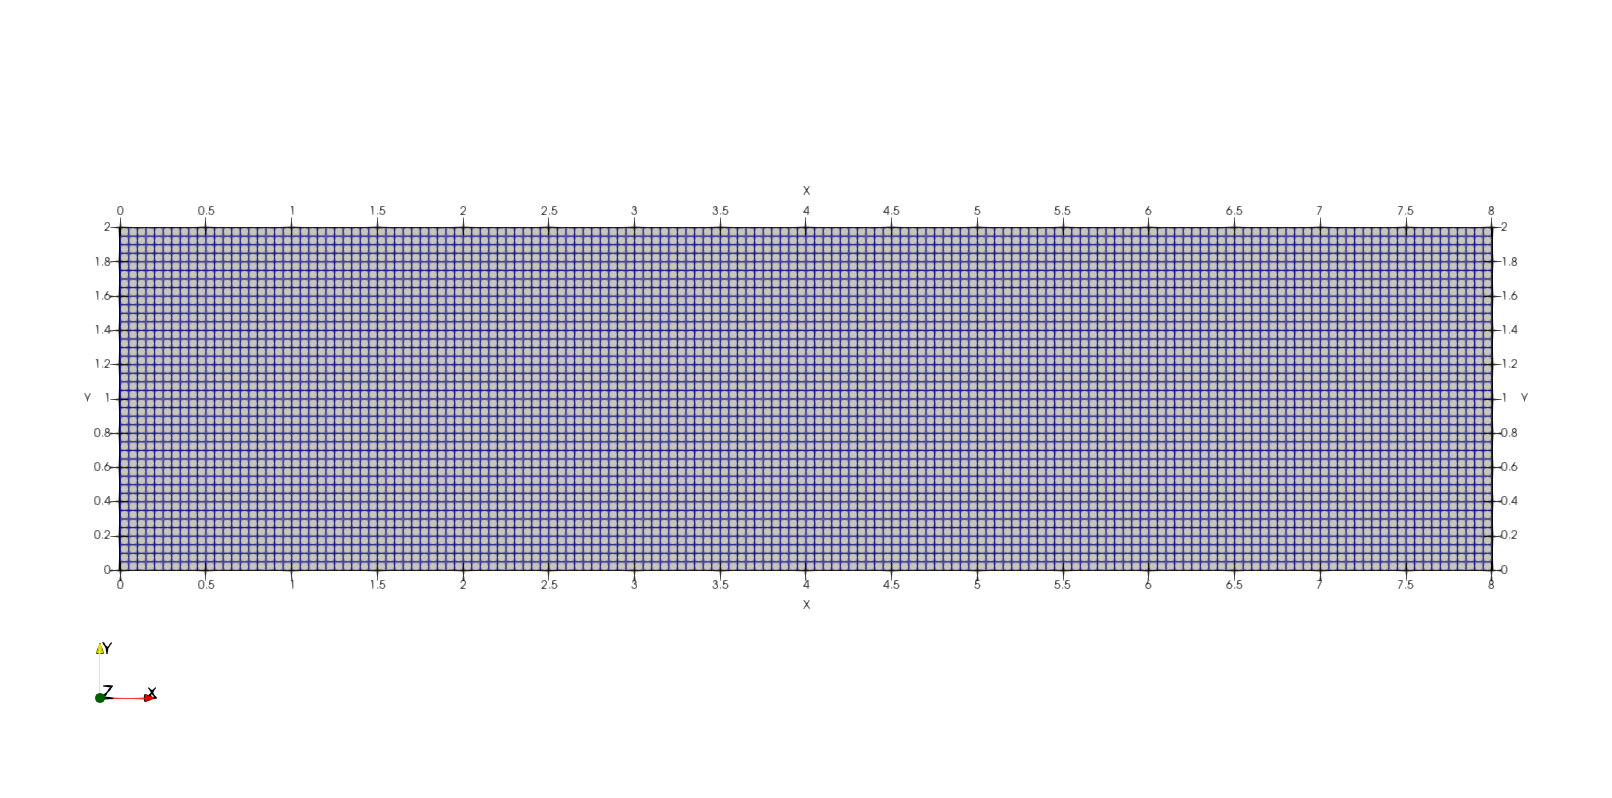
\includegraphics[width=\textwidth]{imgs/ref1.png}
		\end{minipage}
		\captionof{figure}{Exemplo de malha 2D com 1 nível de refinamento.}
	\end{center}
\end{frame}
%----------------------------------------------------------------------------------------------------------------------	



%-------Slide 7-------	
%----------------------------------------------------------------------------------------------------------------------	
\setLayout{vertical}
\begin{frame}[fragile]{}
	\vspace{-1cm}
	\begin{center}
		\begin{minipage}{0.30\textwidth}
			{\footnotesize
				\begin{verbatim}
					0.0 8.0 -1.0 1.0
					2
					0.05 0.05 1
					1 1 160 40
					0.025 0.025 4
					1 1 320 16
					1 65 320 16
					1 17 16 48
					305 17 16 48
				\end{verbatim}
			}
		\end{minipage}
		\hfill
		\begin{minipage}{0.65\textwidth}
			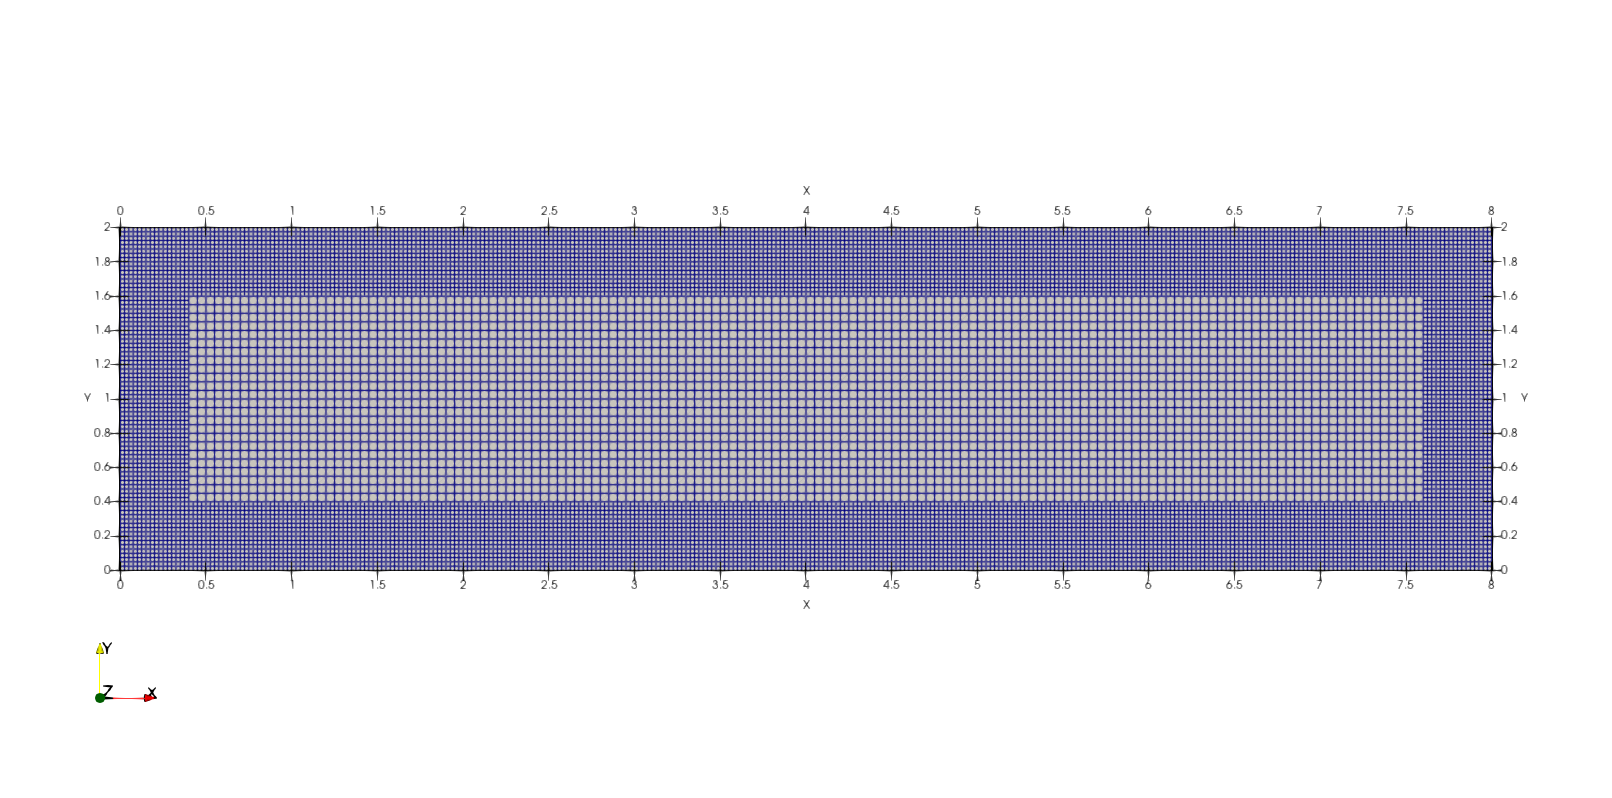
\includegraphics[width=\textwidth]{imgs/ref2.png}
			
			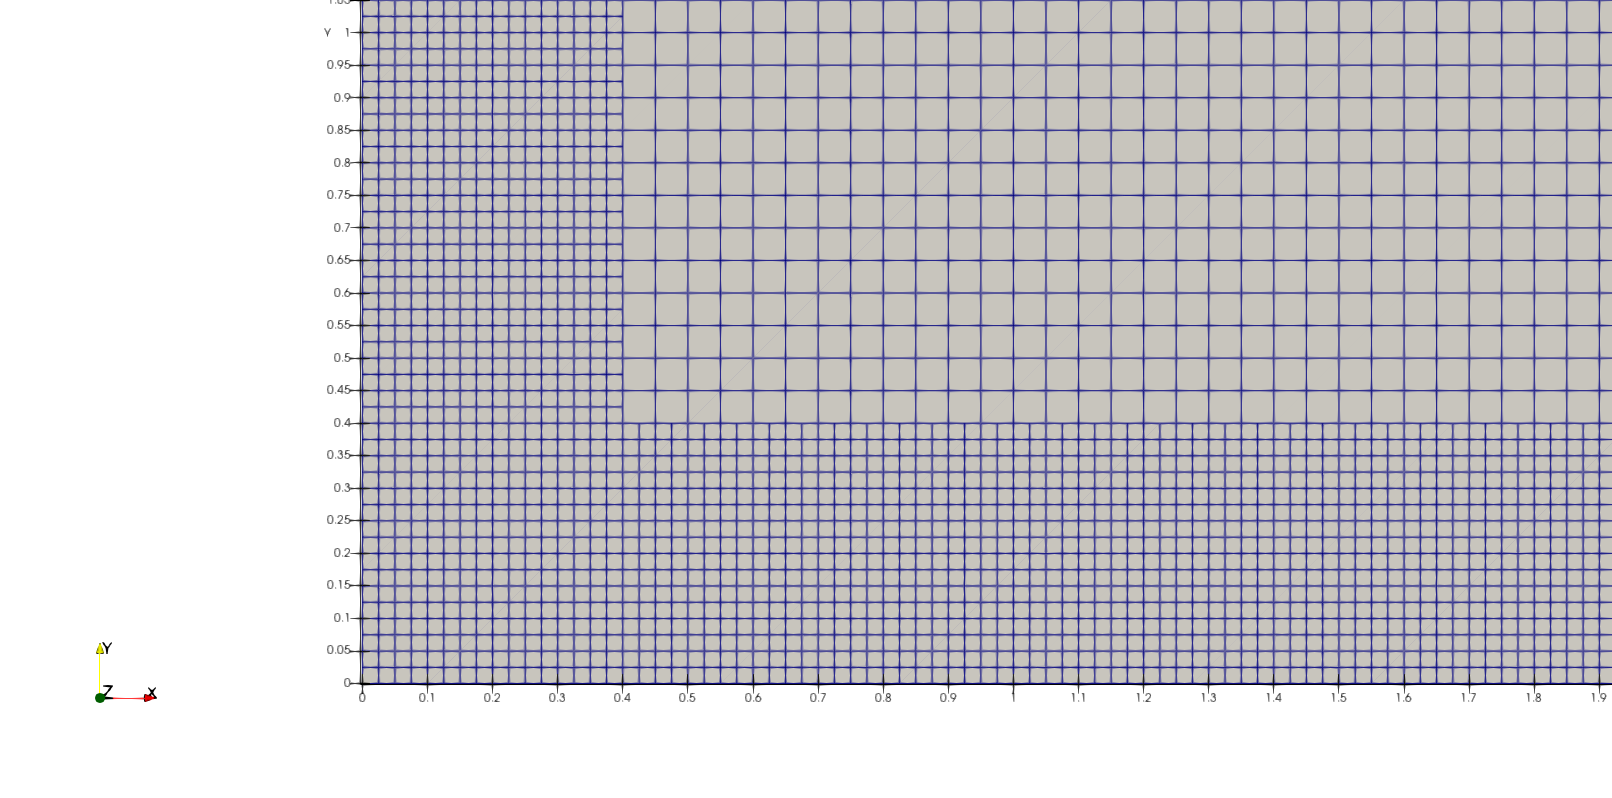
\includegraphics[height=0.3\textheight]{imgs/ref2_border.png}
		\end{minipage}
		\captionof{figure}{Exemplo de malha 2D com 2 níveis de refinamento.}
	\end{center}
\end{frame}
%----------------------------------------------------------------------------------------------------------------------	



%-------Slide 8-------	
%----------------------------------------------------------------------------------------------------------------------	
\setLayout{vertical}
\begin{frame}[fragile]{}
	\vspace{-1.5cm}
	\begin{center}
		\begin{minipage}{0.30\textwidth}
			{\footnotesize
				\begin{verbatim}
					0.0 8.0 -1.0 1.0
					3
					0.05 0.05 1
					1 1 160 40
					0.025 0.025 4
					1 1 320 16
					1 65 320 16
					1 17 16 48
					305 17 16 48
					0.0125 0.0125 4
					1 1 640 16
					1 145 640 16
					1 17 16 128
					625 17 16 128
				\end{verbatim}
			}
		\end{minipage}
		\hfill
		\begin{minipage}{0.65\textwidth}
			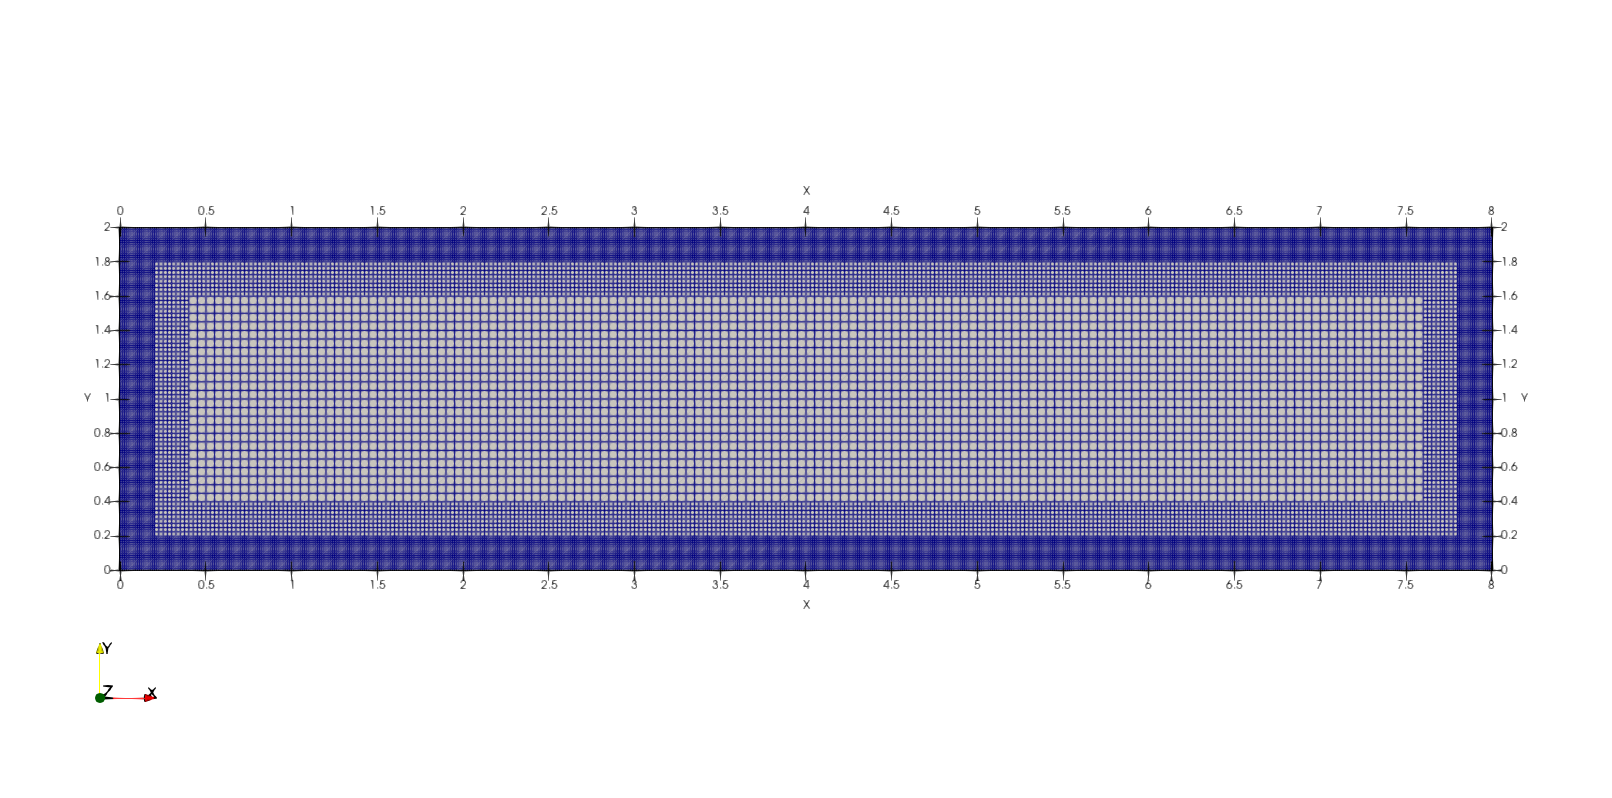
\includegraphics[width=\textwidth]{imgs/ref3.png}
			
			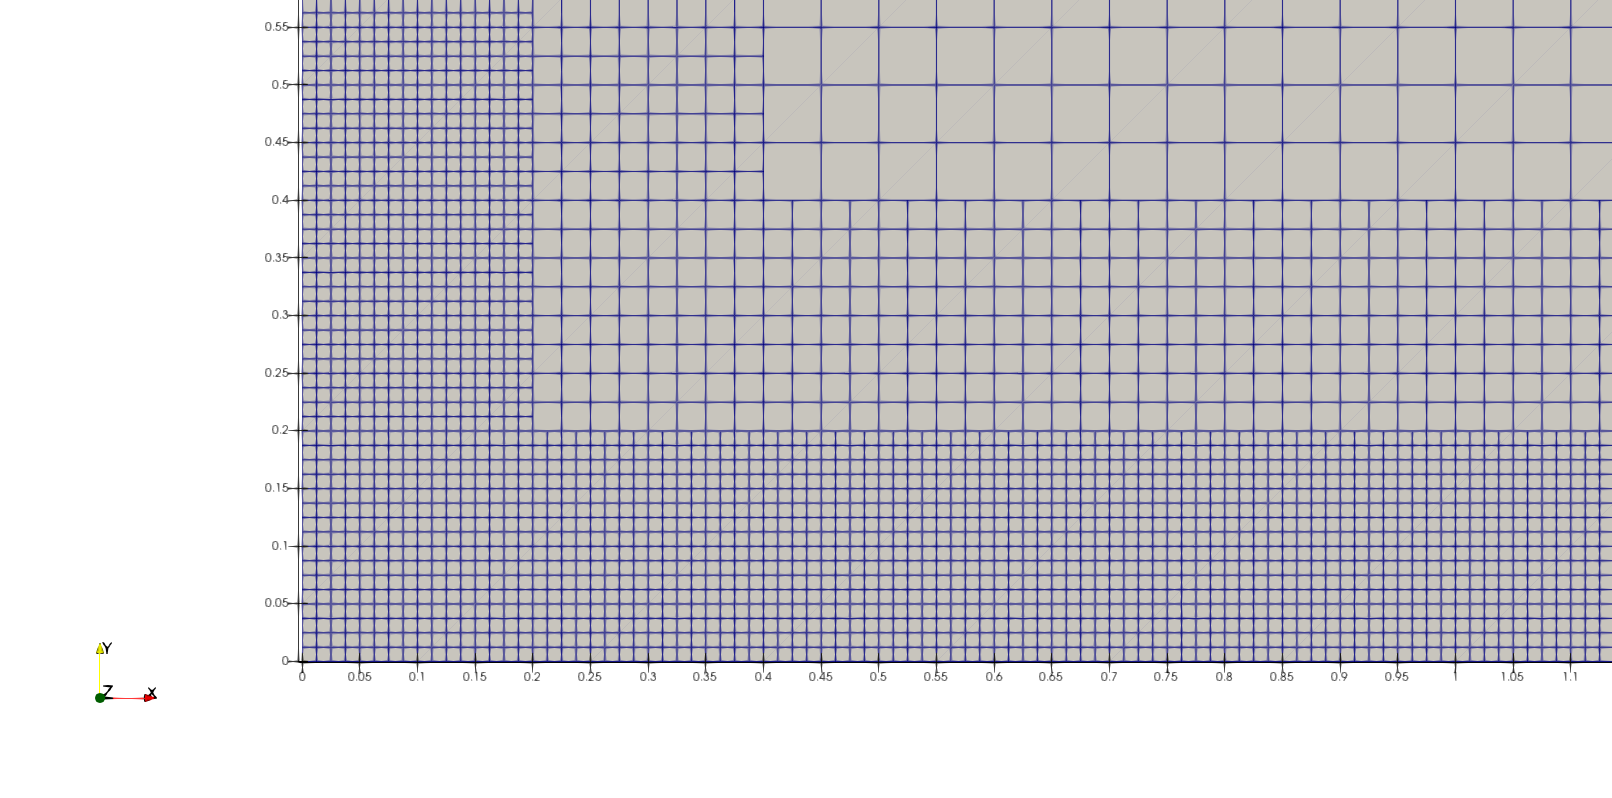
\includegraphics[height=0.35\textheight]{imgs/ref3_border.png}
		\end{minipage}
		\captionof{figure}{Exemplo de malha 2D com 3 níveis de refinamento.}
	\end{center}
\end{frame}
%----------------------------------------------------------------------------------------------------------------------	



%-------Slide 9-------	
%----------------------------------------------------------------------------------------------------------------------	
\setLayout{vertical}
\begin{frame}{}
	\begin{center}
		\begin{minipage}{0.20\textwidth}
			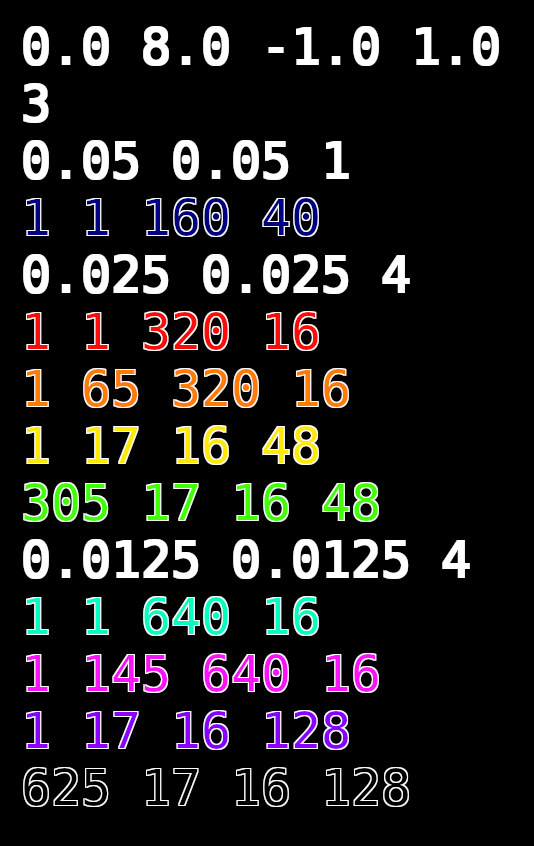
\includegraphics[width=\textwidth]{imgs/ref3_PorPartes_amrColors.png}
		\end{minipage}
		\hfill
		\begin{minipage}{0.75\textwidth}
			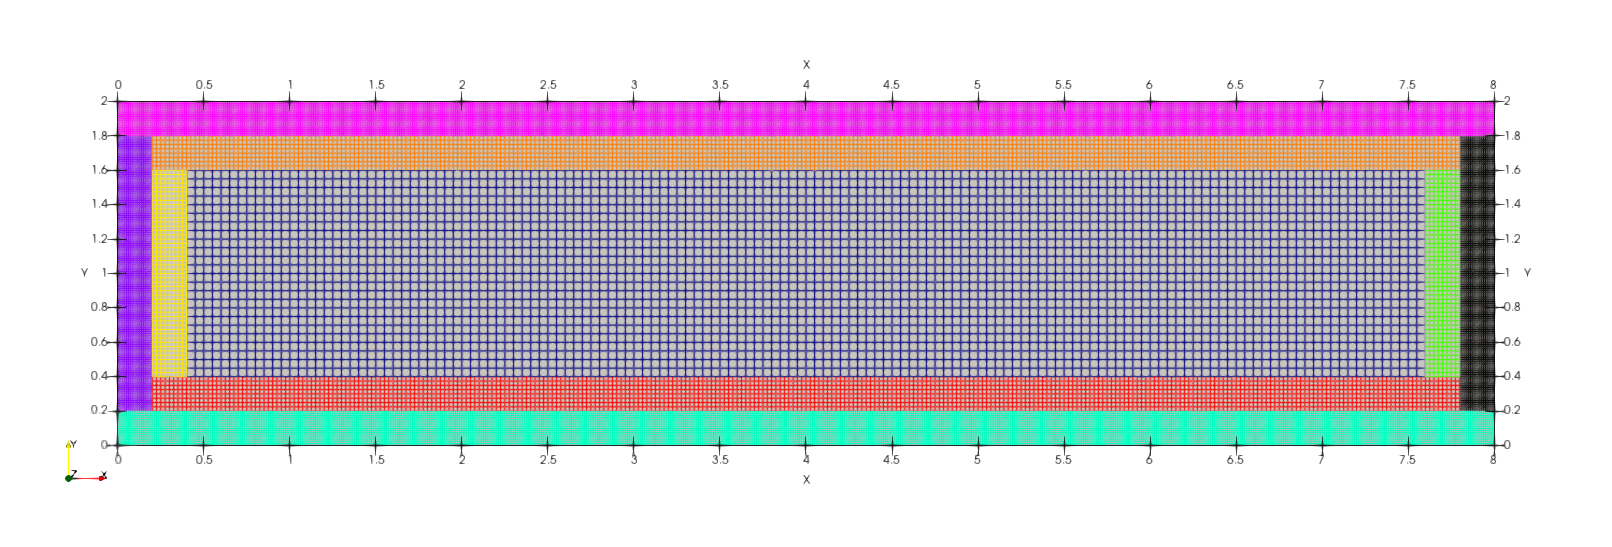
\includegraphics[width=\textwidth]{imgs/ref3_PorPartes.png}
			
			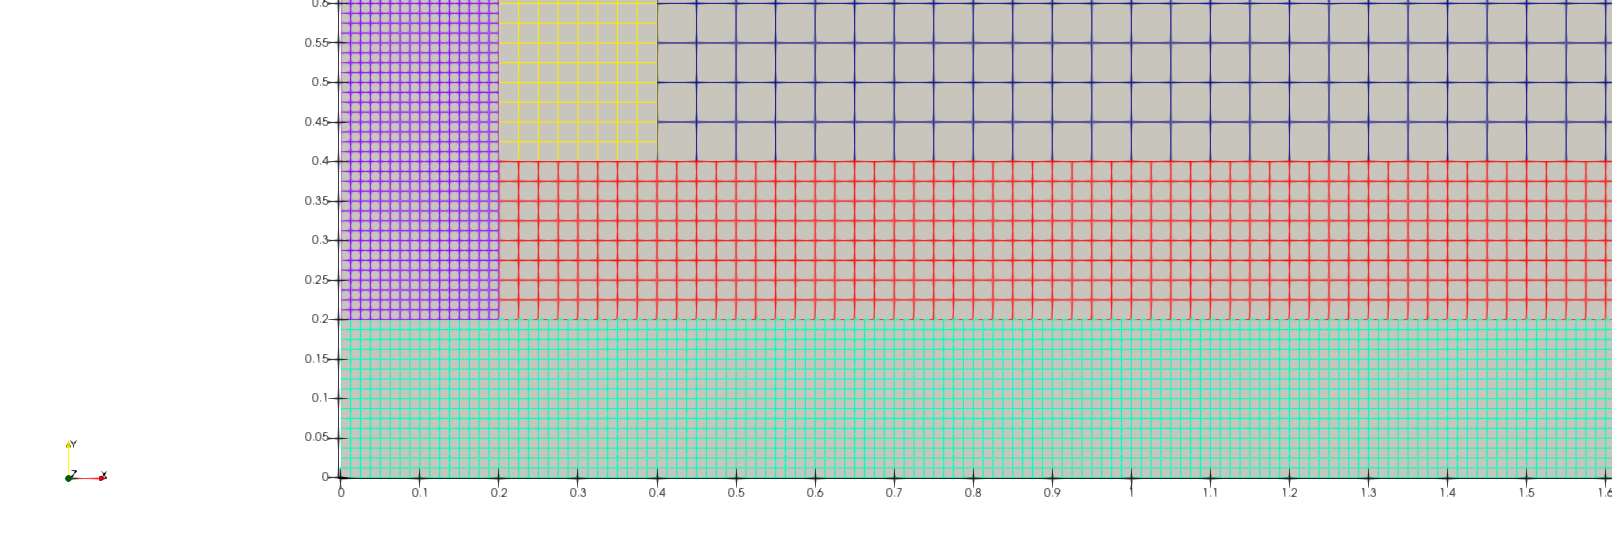
\includegraphics[height=0.3\textheight]{imgs/ref3_PorPartes_border.png}
		\end{minipage}
		\captionof{figure}{Exemplo de malha 2D com 3 níveis de refinamento.}
	\end{center}
\end{frame}
%----------------------------------------------------------------------------------------------------------------------	




\end{document}
%_______________________________________________________________________________________________________________________